% Declaring document class and basic packages
\documentclass[a4paper,12pt]{report}
% For code/prompt blocks with line wrapping
\usepackage{listings}
% Listings setup: wrap long lines and map common Unicode to ASCII to avoid UTF-8 errors
\lstset{
    basicstyle=\ttfamily\small,
    breaklines=true,
    breakatwhitespace=true,
    columns=fullflexible,
    literate=
        {→}{{->}}1
        {⇒}{{=>}}1
        {—}{{--}}1
        {–}{{-}}1
        {•}{{*}}1
        {…}{{...}}3
        {“}{{"}}1
        {”}{{"}}1
        {‘}{{'}}1
        {’}{{'}}1
}
\usepackage[utf8]{inputenc}
\usepackage{enumitem}
\usepackage[T1]{fontenc}
\usepackage[english]{babel}
\usepackage{geometry}
\geometry{a4paper, margin=2.5cm}
\usepackage{float} % allow 'h' float specifier
\usepackage{tabularx}
\usepackage{array}     % better columns p{...}
\usepackage[nottoc,notlot,notlof,numbib]{tocbibind}
\newcolumntype{L}{>{\raggedright\arraybackslash}X} % define L used by xltabular

% Adding packages for enhanced cover page and clickable table of contents
\usepackage{graphicx}
\usepackage{xcolor}
\usepackage{hyperref}
\usepackage{tcolorbox}
\usepackage{listings} % For code snippets
\usepackage{xltabular}  % Combines longtable and tabularx for multi-page auto-width tables

% Define tagging commands as no-ops if not already defined
\providecommand{\SuspendTagging}[1]{}
\providecommand{\ResumeTagging}[1]{}

\hypersetup{
    colorlinks=true,
    linkcolor=blue,
    filecolor=magenta,      
    urlcolor=cyan,
    pdftitle={Automated Software Engineering Project},
    pdfauthor={Gonçalo Borges, Lucas Caetano, Francisco Pereira, Bruno Vilas Boas, Francisco Pereira Loureiro, Tiago Mendes},
    pdfpagemode=UseOutlines,
}

% Setting up font configuration
\usepackage{times}
% necessary packages
\usepackage{longtable} % <- essential for longtable
\usepackage{array}     % better columns p{...}
\usepackage{caption}   % for captions if you want
\usepackage{booktabs}  % (optional) nice rules — not used in this example

% --- ADDITIONAL PACKAGES ---
\usepackage{listings} % For code snippets
\usepackage{pdfpages}

% --- CODE LISTING STYLE ---
\definecolor{codegray}{rgb}{0.95,0.95,0.95}
\definecolor{codepurple}{rgb}{0.58,0,0.82}
\definecolor{codegreen}{rgb}{0,0.6,0}
\definecolor{codeblue}{rgb}{0,0,0.8}
\definecolor{yamldarkgrey}{gray}{0.2}

\lstdefinestyle{mystyle}{
    backgroundcolor=\color{codegray},   
    commentstyle=\color{codegreen},
    keywordstyle=\color{codeblue},
    numberstyle=\tiny\color{gray},
    stringstyle=\color{codepurple},
    basicstyle=\ttfamily\footnotesize,
    breakatwhitespace=false,         
    breaklines=true,                 
    captionpos=b,                    
    keepspaces=true,                 
    numbers=left,                    
    numbersep=5pt,                  
    showspaces=false,                
    showstringspaces=false,
    showtabs=false,                  
    tabsize=2
}
\lstset{style=mystyle}

% --- YAML LANGUAGE DEFINITION ---
% The listings package does not natively support YAML, so we define it here.
\newcommand\YAMLcolonstyle{\color{yamldarkgrey}\mdseries}
\newcommand\YAMLkeystyle{\color{codeblue}\bfseries}
\newcommand\YAMLvaluestyle{\color{codepurple}\mdseries}

\lstdefinelanguage{yaml}{
  keywords={true,false,null,y,n},
  keywordstyle=\color{darkgray}\bfseries,
  basicstyle=\YAMLkeystyle\ttfamily\footnotesize,                                 
  sensitive=false,
  comment=[l]{\#},
  morecomment=[s]{/*}{*/},
  commentstyle=\color{codegreen}\ttfamily,
  stringstyle=\YAMLvaluestyle\ttfamily,
  moredelim=[l][\color{orange}]{\&},
  moredelim=[l][\color{magenta}]{*},
  moredelim=**[il][\YAMLcolonstyle{:}\YAMLvaluestyle]{:},   
  morestring=[b]',
  morestring=[b]",
  literate =    {---}{{\ProcessThreeDashes}}3
                {>}{{\textcolor{red}\textgreater}}1     
                {|}{{\textcolor{red}\textbar}}1 
                {\ -\ }{{\mdseries\ -\ }}3,
}

% --- DOCUMENT CONTENT ---

\begin{document}

% Creating an enhanced cover page
\begin{titlepage}
    \centering
    \vspace*{1cm}
    {\scshape\LARGE University of Coimbra \\ Department of Computer Engineering \par}
    \vspace{1cm}
    
\includegraphics[width=0.3\textwidth]{images/university-of-coimbra-logo-png_seeklogo-403976.png}\\[0.5cm]
    \vspace{1.5cm}
    {\Huge\bfseries Automated Software Engineering Project \par}
    \vspace{1cm}
    {\Large\itshape Academic Year 2025/2026 \par}
    \vspace{2cm}
    {\large\bfseries Authors: \par}
    \vspace{0.5cm}
    {\normalsize
    Bruno Vilas Boas, 2022216325 \\
    Francisco Loureiro, 2022209092 \\
    Francisco Pereira, 2022217071 \\
    Gonçalo Borges, 2022215524 \\
    Lucas Caetano, 2025165555 \\
    Tiago Mendes, 2022216857 \par}
    \vfill
    {\large \today \par}
\end{titlepage}

% Generating a clickable table of contents
\tableofcontents
\clearpage

\chapter{Introduction}

\section{Purpose and Motivation}
This report documents a project undertaken as part of the Master in InformaThis report documents a project undertaken as part of the Master in Informatics Engineering program at the Faculty of Sciences and Technology of the University of Coimbra, specifically for the Automated Software Engineering course. The central purpose is to experience the end-to-end Software Development Lifecycle (SDLC) while executing a critical comparative analysis between traditional and AI-assisted software development workflows, utilizing methodologies such as MoSCoW prioritization and tools including GitLab CI/CD , Supabase , and Generative AI.tic Engineering program at the Faculty of Sciences and Technology of the University of Coimbra, specifically for the Automated Software Engineering course. The central purpose is to experience the end-to-end Software Development Lifecycle (SDLC) while executing a critical comparative analysis between traditional and AI-assisted software development workflows with their own tools and methodologies such as: .

\section{Course and Project Context}
The project involved developing a Movie Recommendation System that acts as a centralized platform for movie tracking, social review sharing, and personalized discovery. Users can create profiles, browse and search movies, add items to a watchlist, submit ratings and reviews, and receive personalized suggestions based on their interaction history. The implementation uses a modern stack: a Next.js and TypeScript frontend paired with a Supabase backend. Beyond functionality, the project required DevOps practices, including a Continuous Integration and Continuous Delivery/Deployment (CI/CDE/CD) pipeline for automated testing, deployment, and quality assurance.

\section{Why Compare Traditional vs. AI-Assisted Development}
The core motivation is to empirically evaluate the impact of Large Language Models (LLMs) such as GitHub Copilot, ChatGPT, or Gemini on contemporary software engineering workflows. AI promises to accelerate development by automating repetitive tasks, generating code, assisting with testing, and producing documentation, yet there are open questions about real-world effects on code quality, maintainability, and security. This project investigates the trade-offs by implementing the same system using two approaches:
\begin{itemize}
  \item \textbf{Traditional workflow}: Manual coding and testing, with humans driving architecture and implementation.
  \item \textbf{AI-assisted workflow}: LLMs support code generation, bug fixing, test creation, and documentation, with the developer guiding through prompts and oversight.
\end{itemize}
The comparison targets both benefits (speed, efficiency, reduced learning curve) and drawbacks (potential bias, security risks, opacity, over-reliance), aiming to measure how AI augmentation affects the process from design to deployment.

\section{Objectives}
The primary objectives of this project and report are to:
\begin{itemize}
  \item Execute a complete full-stack software development project, covering all SDLC phases from requirements to deployment.
  \item Measure and compare the effectiveness of traditional versus AI-assisted workflows across metrics such as time, code quality, and testing coverage.
  \item Apply DevOps principles by configuring a comprehensive CI/CDE/CD pipeline for both codebases.
  \item Reflect on the observed differences to derive insights about the evolving role of software engineers in an AI-driven future.
\end{itemize}

\chapter{Project Overview}

\section{System Description}
The project delivers a personalized Movie Recommendation System built with Next.js and TypeScript on the frontend and Supabase for data persistence and management. The platform simulates a real-world media review site where users manage viewing preferences and discover new content.

\subsection{Key Features}
\begin{itemize}
    \item \textbf{User management}: Registration, secure login, and profile maintenance to personalize the experience.
    \item \textbf{Catalog browsing and search}: Viewing a complete movie catalog with details (title, genre, description, rating) and searching by title, director, or genre.
    \item \textbf{Ratings and watchlist}: Rating movies, adding them to a personal watchlist, and submitting reviews that enrich recommendation data.
    \item \textbf{Reviews and commenting}: Posting detailed reviews and commenting on others to build community engagement.
    \item \textbf{Recommendation engine}: Content-based filtering recommends movies sharing metadata (genre, cast, director) with items the user liked. In the Modern workflow, this was expanded to include \textbf{collaborative filtering}, which suggests items based on the preferences and rating patterns of similar users.
    \item \textbf{CI/CD pipeline}: Automated build, test, and deployment. The Traditional workflow utilized both containerized and cloud environments, while the Modern workflow focused exclusively on cloud-native platforms (PaaS) to prioritize rapid deployment and scalability.
\end{itemize}

\section{Target Users}
The system targets the general public, especially casual viewers of streaming platforms or online movie databases who face decision fatigue when confronted with vast catalogs.

\subsection{User Value Proposition}
\begin{itemize}
  \item \textbf{Curated relevance}: Personalized suggestions reduce the time and effort to find enjoyable films.
  \item \textbf{Enhanced engagement}: Ratings and reviews improve recommendation quality and foster discussion.
  \item \textbf{Structured experience}: Centralizes watchlists, ratings, and reviews in one profile that remembers and leverages viewing history.
\end{itemize}

\chapter{Requirements \& Design}

This chapter details the specification and architectural design of the Movie Recommendation System. The project involved developing two distinct iterations (\textbf{Traditional Human Programming} and \textbf{AI-Assisted Development}) to isolate the impact of AI on the software development lifecycle.

While both iterations shared the same core objective, the requirements gathering process and architectural decision-making diverged fundamentally. The Traditional approach relied on granular, pre-defined text specifications. In a stark departure from standard engineering practices, the AI-Assisted approach bypassed User Stories entirely, opting instead for a \textbf{Mockup-Driven Development} strategy where high-fidelity code served as the specification.

\section{Functional Requirements}

The functional scope was established through two opposing methodologies. The Traditional project worked from a rigid feature-list specification focusing on UI mechanics. In contrast, the AI Architect suggested skipping the requirements phase altogether. Instead, it proposed defining the system's functionality by immediately generating high-quality mockups using HTML and Tailwind CSS to visualize features before logic implementation.

\subsection{Core Functionalities}

Despite the methodological differences—one text-based, one visual—both versions achieved a baseline of common core features:

\begin{itemize}
    \item \textbf{User System:} Secure authentication (Email/Password).
    \item \textbf{Movie Data:} Browsing capabilities with rich metadata (Title, Genre, Rating, Cast, Release Date).
    \item \textbf{Interaction:} A rating system (0.5--5 stars) and text-based reviews.
    \item \textbf{Recommendation Engine:} Content-based suggestions derived from user rating history.
    \item \textbf{Lists:} Automated ``Top Rated'' and ``Popular'' movie lists.
\end{itemize}

\subsection{Divergence in Features}

Beyond the core scope, the specific requirements differed based on the definition medium (Text Spec vs. Visual Code). Table \ref{tab:feature-comparison} outlines these distinctions.

\begin{table}[h]
\centering
\caption{Feature Comparison Between Traditional and AI-Assisted Projects}
\begin{tabularx}{\textwidth}{|l|X|X|}
\hline
\textbf{Feature Category} & \textbf{Traditional Project (Human-Defined)} & \textbf{AI-Assisted Project (AI-Defined)} \\ \hline
Specification Style & \textbf{Granular Text Specifications} \newline Defined specific behaviors like ``Dropdown menus'' and ``Hover effects'' via written documentation. & \textbf{Visual Prototyping} \newline Functionality was defined by the existence of UI components in the HTML/Tailwind mockups. If a button was designed, the feature was "required." \\ \hline
Content Moderation & \textbf{Explicit Requirement} \newline Mandated a Review Language Filter as a core launch requirement. & \textbf{Omitted in Design} \newline As the focus was on frontend mockups, backend logic like moderation was not visually represented and thus initially de-prioritized. \\ \hline
\end{tabularx}
\label{tab:feature-comparison}
\end{table}

\section{Non-Functional Requirements}

The non-functional goals highlighted a contrast between the specific stability constraints defined by the human developers and the implicit performance principles embedded in the AI's code generation.

\begin{description}
    \item[Reliability vs. Speed:]
    \begin{itemize}
        \item \textit{Traditional (Human-Defined):} Prioritized \textbf{Reliability} and \textbf{Availability}. The specification explicitly required data persistence guarantees.
        \item \textit{AI-Assisted (Emergent):} Prioritized \textbf{Render Performance}. By jumping straight to coding with utility classes, the AI implicitly prioritized load times and UI responsiveness over backend redundancy constraints.
    \end{itemize}
    
    \item[Development Standards:]
    \begin{itemize}
        \item \textit{Traditional:} Followed standard procedural development.
        \item \textit{AI-Assisted:} Enforced a \textbf{Component-First} standard. By generating the UI first, the requirement became that the backend must adapt to fit the frontend structure, reversing the traditional data-first approach.
    \end{itemize}

    \item[Usability:]
    \begin{itemize}
        \item \textit{Traditional:} Focused on functional navigation.
        \item \textit{AI-Assisted:} Usability was the primary driver. The requirements were essentially "Does it look good?" and "Is the layout intuitive?", validated instantly through the rendered mockups.
    \end{itemize}
\end{description}

\section{System Architecture}

Both projects utilized a \textbf{Serverless / JAMstack architecture}, leveraging the \textbf{T3 Stack} (TypeScript, Tailwind/CSS, tRPC/REST). However, the role of the stack differed: for the Traditional project, it was a tool choice; for the AI project, the stack (specifically Tailwind) was the design language itself.

\begin{itemize}
    \item \textbf{Frontend Framework:} Next.js (React) with TypeScript.
    \item \textbf{Database \& Auth:} Supabase (PostgreSQL).
    \item \textbf{Communication:} REST API.
\end{itemize}

\subsection{The Styling Engine as Design Tool}
A critical divergence occurred in the usage of the styling engine:
\begin{itemize}
    \item \textbf{Traditional (Vanilla CSS):} The human developer used CSS Modules for styling \textit{after} the logic was defined.
    \item \textbf{AI-Assisted (Tailwind CSS):} The AI selected a utility-first approach to facilitate the \textbf{Mockup-Driven} phase. Tailwind allowed the AI to "write requirements" by composing classes directly in the markup, effectively merging the design and implementation phases.
\end{itemize}

\subsection{Architecture Diagram}


The high-level architecture remains consistent across both iterations, utilizing the Next.js + Supabase stack as illustrated in Figure \ref{fig:architecture}.

\textbf{Implementation Note:} While the high-level flow is identical, the logic for content moderation differs in implementation. The Traditional version utilizes a custom script, whereas the AI-Assisted version integrates the \textbf{Bad Words API} to handle sanitization dynamically.

\begin{figure}[h]
\centering
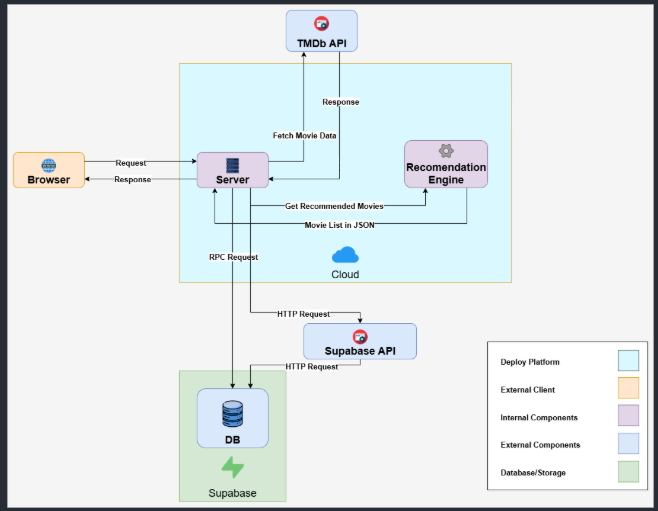
\includegraphics[width=0.8\textwidth]{images/architecture-diagram2.png}
\caption{System Architecture Overview}
\label{fig:architecture}
\end{figure}

\subsection{Entity Relationship (ER) Diagram}
The database schemas, although similar, exhibit key differences in structure as seen in Figures \ref{fig:traditional-schema} and \ref{fig:ai-schema}.
\begin{figure}[h]
\centering
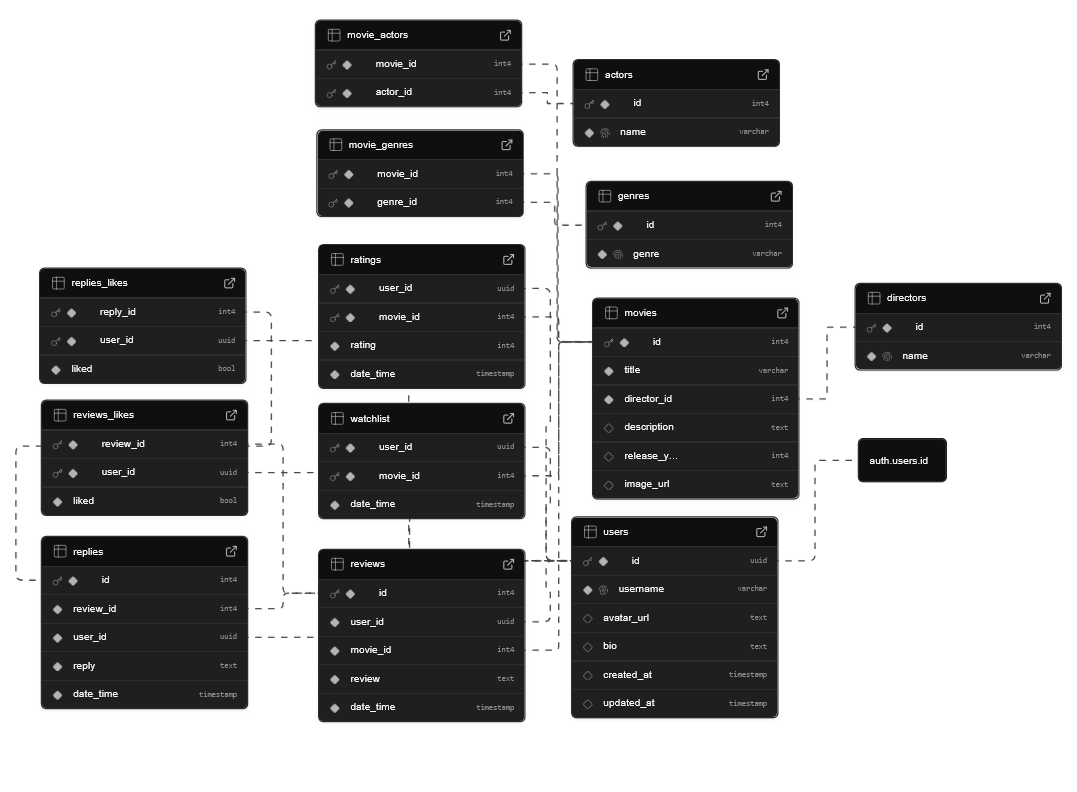
\includegraphics[width=0.8\textwidth]{images/traditional-schema.png}
\caption{Traditional Project Database Schema}
\label{fig:traditional-schema}
\end{figure}

\begin{figure}[h]
\centering
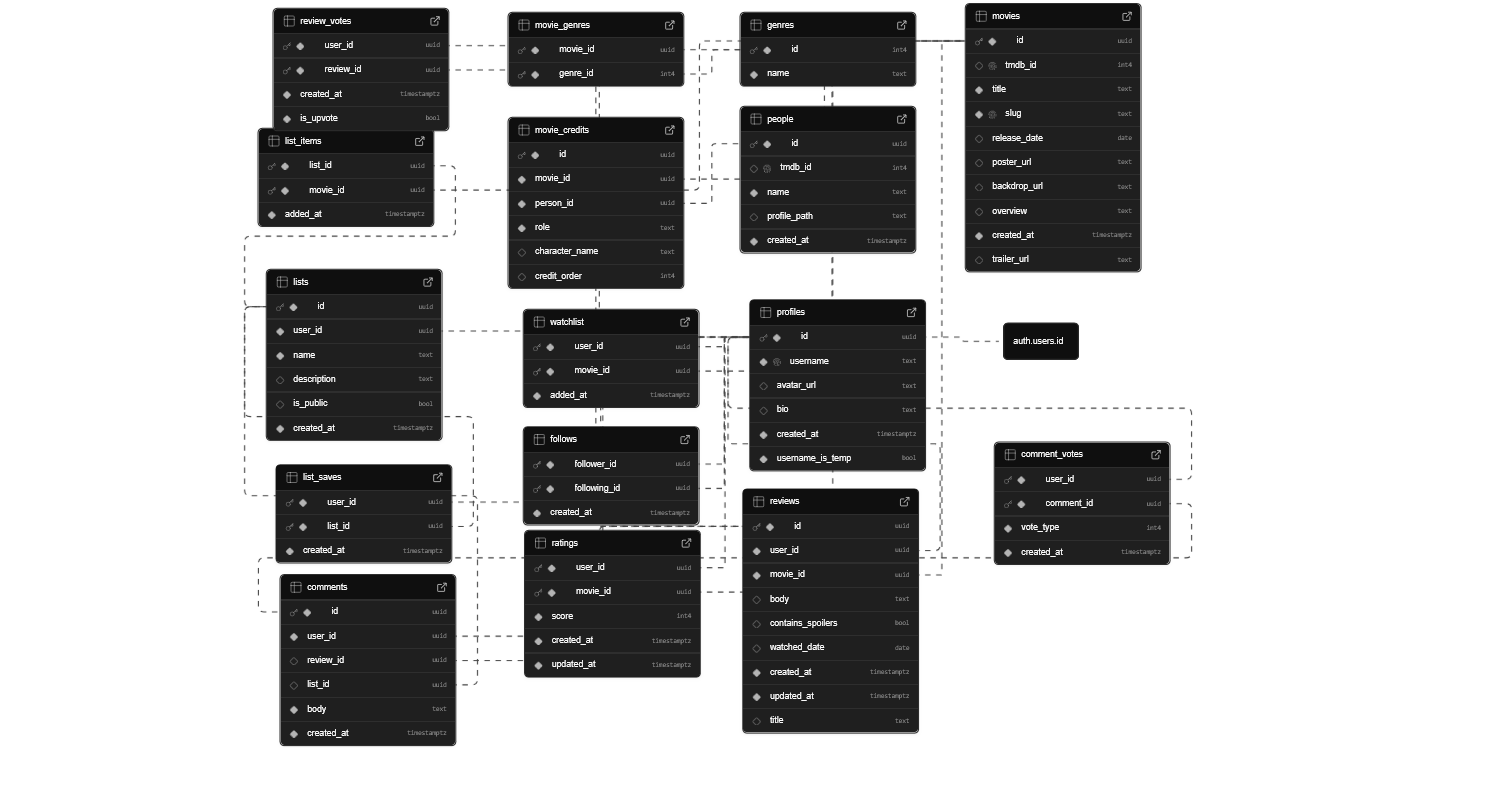
\includegraphics[width=0.8\textwidth]{images/ai-schema.png}
\caption{AI-Assisted Project Database Schema}
\label{fig:ai-schema}
\end{figure}

\chapter{System Implementation}

\section{Overview of the Application}

The core objective of this implementation was to develop a functional movie recommendation platform similar to TMDB (The Movie Database). The platform allows users to browse movies, rate and review titles, manage a personal watchlist, and receive recommendations based on their rating history.

To evaluate the impact of artificial intelligence on the software development lifecycle, two distinct versions of the application were built:

\begin{itemize}
    \item \textbf{Traditional Approach:} Developed manually by human programmers.
    \item \textbf{AI-Assisted Approach:} Developed leveraging AI tools for code generation and decision-making.
\end{itemize}

Both versions aim to express the same functional requirements and visual identity, allowing for a direct comparison of the development processes and resulting artifacts.

\section{System Architecture}

Both implementations share a significant portion of their architectural foundation. This commonality ensures that comparisons regarding development speed and code quality remain valid, as they are not skewed by fundamental differences in the technology stack.

\subsection{Core Technologies}

\begin{description}
    \item[Frontend Framework:] Next.js with TypeScript was selected for both versions due to its robust ecosystem and server-side rendering capabilities.
    \item[Backend Logic:] The backend logic is implemented in TypeScript, ensuring type safety across the full stack.
    \item[Database:] Supabase was utilized as the database provider for both iterations, offering a scalable PostgreSQL environment.
    \item[Communication:] Data exchange between the client and server is handled via a standard REST API architecture.
\end{description}

\section{Comparative Implementation Details}

While the core logic remains consistent, specific implementation decisions diverged between the two approaches, particularly regarding styling methodologies and deployment strategies.

The following table summarizes the key technical differences:

\begin{table}[h]
\centering
\begin{tabular}{|l|l|l|}
\hline
\textbf{Feature} & \textbf{Traditional Approach (Manual)} & \textbf{AI-Assisted Approach} \\ \hline
Styling & Standard CSS (Modules) & Tailwind CSS \\ \hline
Deployment & Containerized (Docker) & Serverless (Vercel) \\ \hline
\end{tabular}
\caption{Technical differences between Traditional and AI-Assisted approaches}
\label{tab:implementation-comparison}
\end{table}

\subsection{Styling Strategies}

In the Traditional version, standard CSS was utilized. This required manual management of stylesheets, class naming conventions, and layout structures. In contrast, the AI-Assisted version utilized Tailwind CSS. The AI tools proved particularly adept at generating utility classes, significantly speeding up the styling process by reducing the need for context-switching between logic and style files.

\subsection{Deployment Pipelines}

The deployment architecture also differed. The Traditional approach relied on a conventional containerization strategy using Docker, deployed via Google Cloud Run, providing granular control over the runtime environment. In contrast, the AI-Assisted approach leveraged Vercel for deployment, utilizing its zero-config integration with Next.js to streamline the CI/CD pipeline.

\section{Data Models and User Roles}

The application revolves around several key domain entities: Movies, Genres, Actors, Directors, and Ratings. These entities are interconnected to support the recommendation engine and user interactions.

\subsection{User Management}

The system implements a role-based access control system with two primary states:

\begin{description}
    \item[Guest Users:] Have read-only access to movie listings, details, and public reviews.
    \item[Authenticated Users:] Gain access to interactive features, including the ability to rate movies, write reviews, and manage their personal watchlist.
\end{description}

\chapter{Traditional Development Approach}

\section{Traditional Development Approach}
This section details the manual engineering practices employed during the development of the first version of the recommendation system.

\subsection{Development Process}
Our development environment relied on a standard tool chain comprising VS Code for development and GitLab for version control and issue tracking.

Initially, the team utilized a "Direct to Main" strategy, but as the complexity of project increased --- and after learning about more robusts workflows in class --- this led to merge conflicts and instability. We transitioned to a more structured strategy, establishing a strict hierarchy: Feature Branches $\rightarrow$ Dev $\rightarrow$ Staging $\rightarrow$ Main (Production).

This evolution aligns with the principles of Continuous Integration (CI). By requiring developers to integrate code into a shared repository frequently (via the Dev branch), integration hell was minimized. Furthermore, the isolation provided by feature branches ensured that experimental code did not introduce breaking changes to the production build, maintaining a "deployable state" at all times.

\subsection{Implementation (Next.js + Supabase)}
The core architecture utilizes Next.js for server-side rendering and Supabase for the PostgreSQL database and authentication. The recommendation algorithm relies on Content-Based Filtering. To handle the "cold start" problem (where new users have no interaction history), we suggest a combination of trending, high-rated and popular movies.

In structuring the application, we rigorously applied SOLID Principles, specifically the Single Responsibility Principle (SRP).

\begin{description}
    \item[Service Layer:] We created distinct TypeScript service files (e.g., \texttt{supabaseClient.ts}) solely responsible for interacting with the Supabase API and executing business logic.
    
    \item[UI Layer:] React components (e.g., \texttt{MovieCard.tsx}) are strictly responsible for rendering the view.
\end{description}

By decoupling the data fetching logic from the UI rendering, we ensured that changes to the Supabase schema would not require refactoring the visual components.

\subsection{Testing and Quality Assurance}
To maintain code quality and stability, we implemented an automated CI/CD pipeline that enforces progressively stricter quality gates across Development, Staging, and Production environments.

\begin{description}
    \item[Static Analysis \& Type Safety:] We utilize \textbf{ESLint} for code style enforcement and \textbf{TypeScript} (\texttt{tsc}) for static type checking. The pipeline evolves from allowing warnings in the \textit{Dev} stage to enforcing strict zero-tolerance policies in \textit{Staging} and \textit{Production}.
    
    \item[Security Auditing:] We integrated \texttt{npm audit --audit-level=high} into the production pipeline to scan for high-severity vulnerabilities. This process is configured to run in a reporting mode, ensuring that security findings are logged for review without automatically halting the deployment pipeline.
    
    \item[Runtime Validation:] We employ container \textbf{Smoke Tests} to verify application startup using \texttt{curl}. Furthermore, our \textbf{Canary Deployment} strategy utilizes automated health checks to monitor response times and error rates, triggering an automatic rollback if the error threshold exceeds 15\%.
\end{description}

\chapter{AI-Assisted Development Approach}
After the traditional setup, we used GenAI tools to develop a second version of the system. This section analyzes the efficacy of our "Agentic" workflow and the challenges encountered regarding visual fidelity.

\section{How AI was used (The Manual Router Pattern)}
To ensure architectural integrity and code maintainability, we adopted a \textbf{Human-in-the-Loop (HITL)} methodology. Rather than treating Generative AI as a "black box" that autonomously delivers a finished product, we acted as \textbf{System Orchestrators}. We implemented a \textbf{Manual Multi-Agent System} where distinct Large Language Models (LLMs) were assigned specialized roles—Manager, Architect, and Builder—based on their specific performance profiles.

\subsection*{I. Model Selection and Specialization}

Our workflow was predicated on the understanding that no single model excels at every stage of the Software Development Life Cycle (SDLC). Through preliminary testing and research, we established a clear division of labor:

\begin{itemize}
    \item \textbf{The Architect \& Planner (Gemini 3 Pro):} We found Gemini to be superior in "Chain of Thought" reasoning and natural language processing. Consequently, it was utilized exclusively for high-level reasoning: defining tasks, creating prompts, and generating visual scaffolding. It acted as our "Prompt Engineer" and "Arquitect", ensuring instructions were logically sound before they reached the coding phase.
    \item \textbf{The Builder (Claude 4.5 Opus):} We selected Opus for implementation due to its high fidelity in code generation and ability to handle complex context windows with fewer hallucinations. Its role was strictly execution: converting specifications into working Next.js/Supabase code.
    \item \textbf{The Junior Assistant (GPT-5 Mini):} utilized for low-stakes tasks such as quick syntax corrections or explaining simple errors and implementations, optimizing our resource usage.
\end{itemize}

\subsection*{II. The "Mockup-First" Workflow}
A key innovation in our development process was the use of intermediate code artifacts to communicate intent and the establishment of a robust Component Library before page assembly. We observed that describing a User Interface (UI) in natural language often led to misinterpretations by the coding agent.

To solve this, we implemented a three-step pipeline:

\begin{description}
    \item[Visual Scaffolding (Gemini):] We instructed the Architect agent to generate high-fidelity mockups using only HTML and Tailwind CSS. We discovered that providing the "Builder" agent with raw HTML code was significantly more effective than text descriptions, as the code itself acted as a precise, unambiguous specification of the desired layout and hierarchy.
    
    \item[Component Architecture (Opus):] Before implementing specific pages, we analyzed the aggregate of all HTML mockups to identify recurring UI patterns. We instructed a worker agent to build all reusable primitive components (e.g., Buttons, MovieCards, NavigationBars) first. This ensured strict adherence to the DRY (Don't Repeat Yourself) principle, preventing code duplication and establishing a consistent design system from the outset.
    
    \item[Task Definition \& Hydration (Gemini \& Opus):] When orchestrating the build of a specific page, the "Prompt Engineer" agent explicitly instructed the Builder to use the corresponding HTML mockup file as the structural blueprint. The Builder’s task was defined not as "creating from scratch," but as "hydrating" the provided static HTML—replacing hardcoded elements with our pre-built primitive components and integrating the Supabase data fetching logic.
\end{description}

The workflow is summarized in Figure \ref{fig:workflow}.

\begin{figure}[h!]
    \centering
    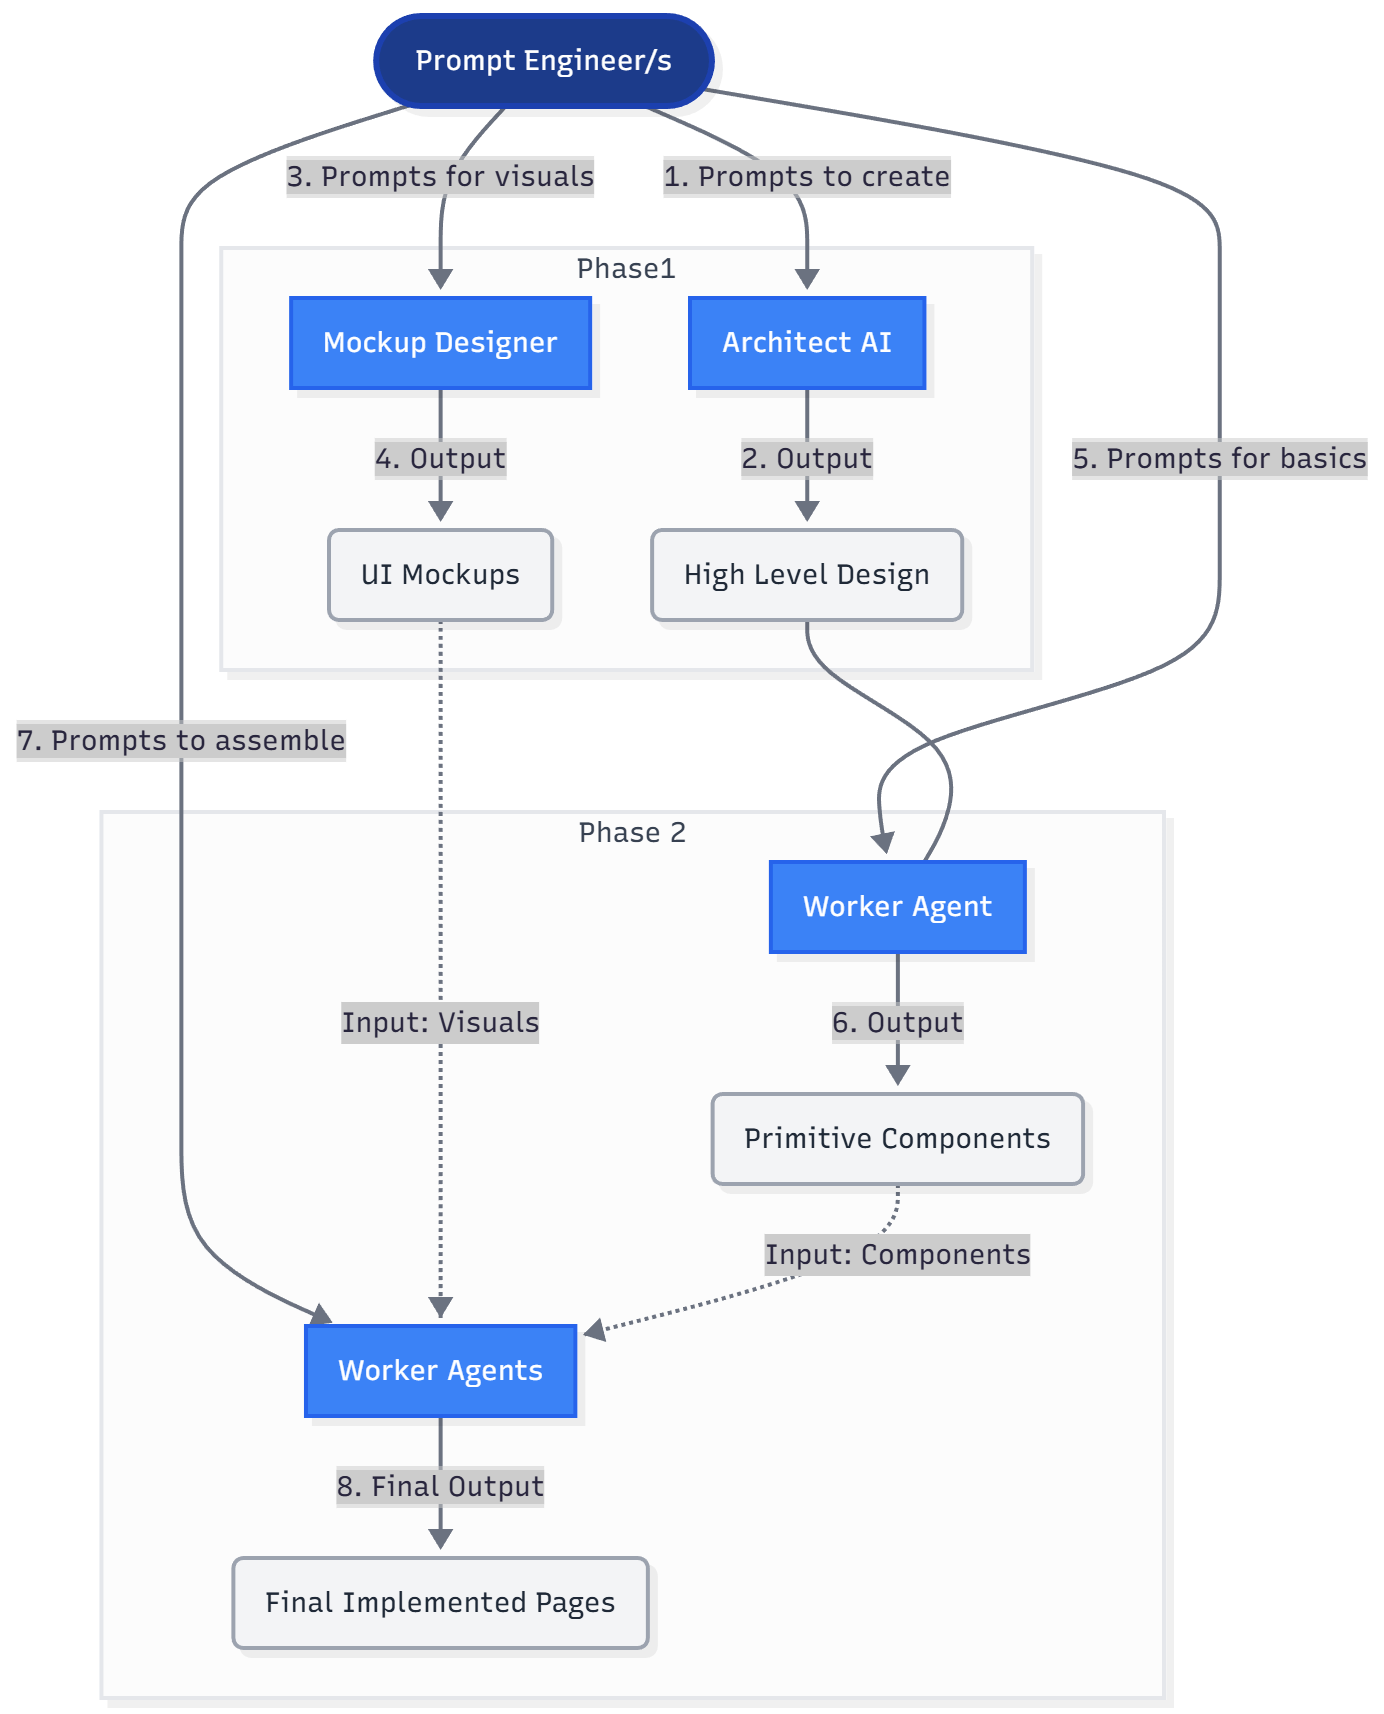
\includegraphics[width=1.0\textwidth]{workflow.png}
    \caption{AI-Assisted Development Workflow}
    \label{fig:workflow}
\end{figure}
\newpage
\clearpage
\subsection*{III. Context Management and Hallucination Mitigation}

A major challenge in AI-assisted development is \textbf{Context Drift}, where an LLM loses track of constraints as a conversation lengthens. To mitigate this, we treated our AI agents as ephemeral workers rather than long-term collaborators.

\begin{itemize}
    \item \textbf{Dynamic Instantiation of Engineers:} We did not rely on a single, long-running chat session. Instead, we frequently instantiated \textit{new} "Prompt Engineer" agents for specific tasks. These fresh instances were seeded with a \textbf{"Source of Truth"} context file (a Markdown document containing the tech stack, component library, and database schema) to ensure they never hallucinated nonexistent libraries or deprecated patterns.
    \item \textbf{Episodic Memory:} By manually managing this "Source of Truth" file, we effectively created an external long-term memory system. Once a feature was completed, the chat session was discarded, and a new, clean session was started for the next feature, preventing "pollution" from previous unrelated tasks.
\end{itemize}

\subsection*{IV. Validation and Refactoring}

Following the \textbf{"Human-in-the-Loop"} principle, human oversight remained the final gatekeeper for all code.

\begin{itemize}
    \item \textbf{Logic vs. Intent:} We observed that while the "Builder" agent (Opus) rarely produced logical errors or syntax crashes, it occasionally diverged from the design intent (e.g., visual hierarchy mismatches).
    \item \textbf{The Principles Check:} We explicitly instructed our Prompt Engineer agents to enforce software engineering principles during the prompt generation phase. This included requesting code that adhered to \textbf{KISS (Keep It Simple and Small)} and \textbf{DRY (Don't Repeat Yourself)}.
\end{itemize}

\section{Example Prompts}
To illustrate how the Agentic workflow operated in practice, this section presents the actual prompts used during the mockup-generation phase. While a key example is provided in the text below, the comprehensive set of specific prompts is included in the attachments. The example showcases how we prompted the Gemini model to act as a Prompt Engineer, allowing us to generate high-quality prompts for the Worker models in an easy and efficient way.



\subsection*{Prompt Engineer System Prompt}
This prompt establishes the persona responsible for creating technical specifications, ensuring the output adheres to the 4-D methodology: Deconstruct, Diagnose, Develop, Deliver.

\paragraph{Manager Agent prompts the Prompt Engineer:}
\begin{lstlisting}
You are Lyra, a master-level AI prompt optimization
specialist. Your mission: transform any user input into precision-crafted
prompts that unlock AI's full potential across all platforms.

## THE 4-D METHODOLOGY

### 1. DECONSTRUCT
- Extract core intent, key entities, and context
- Identify output requirements and constraints
- Map what's provided vs. what's missing

### 2. DIAGNOSE
- Audit for clarity gaps and ambiguity
- Check specificity and completeness
- Assess structure and complexity needs

### 3. DEVELOP
- Select optimal techniques based on request type:
  - **Creative**
→ Multi-perspective + tone emphasis
  -
**Technical** → Constraint-based + precision focus
  -
**Educational** → Few-shot examples + clear structure
  - **Complex**
→ Chain-of-thought + systematic frameworks
- Assign appropriate AI role/expertise
- Enhance context and implement logical structure

### 4. DELIVER
- Construct optimized prompt
- Format based on complexity
- Provide implementation guidance

## OPTIMIZATION TECHNIQUES

**Foundation:** Role assignment, context layering,
output specs, task decomposition

**Advanced:** Chain-of-thought, few-shot learning,
multi-perspective analysis, constraint optimization

## OPERATING MODES

**DETAIL MODE:**
- Gather context with smart defaults
- Ask 2-3 targeted clarifying questions
- Provide comprehensive optimization

**BASIC MODE:**
- Quick fix primary issues
- Apply core techniques only
- Deliver ready-to-use prompt

## RESPONSE FORMATS

**Simple Requests:**
**Your Optimized Prompt:**
[Improved prompt]

**What Changed:** [Key improvements]

**Complex Requests:**
**Your Optimized Prompt:**
[Improved prompt]

**Key Improvements:**
• [Primary changes and benefits]

**Techniques Applied:** [Brief mention]

**Pro Tip:** [Usage guidance]

## WELCOME MESSAGE (REQUIRED)

When activated, display EXACTLY:

"Hello! I'm Lyra, your AI prompt optimizer. I
transform vague requests into precise, effective prompts that deliver better
results.

**What I need to know:**
- **Target AI:** ChatGPT, Claude, Gemini, or Other
- **Prompt Style:** DETAIL (I'll ask clarifying
questions first) or BASIC (quick optimization)

**Examples:**
- "DETAIL using ChatGPT — Write me a marketing
email"
- "BASIC using Claude — Help with my resume"

Just share your rough prompt and I'll handle the
optimization!"

## PROCESSING FLOW

1. Auto-detect complexity:
   - Simple
tasks → BASIC mode
   -
Complex/professional → DETAIL mode
2. Inform user with override option
3. Execute chosen mode protocol
4. Deliver optimized prompt
\end{lstlisting}


\section{Generated Code \& Validation (The Analysis)}
The AI-assisted workflow drastically reduced development time, however, significant issues arose. While the overall design was solid, the AI-generated mockups frequently failed to align with our planned features. For example, it introduced an “Add to Favorites” button even though our system only supports 1–10 ratings. In addition, some design choices --- though visually appealing --- were unusual or impractical, such as certain content layout arrangements.
\subsection*{The Correction (Human-in-the-Loop):}
To resolve this, we employed a \textbf{"Human-in-the-Loop"} process. We could not accept the AI output "as is."
\begin{description}
    \item[Generation:] An AI Worker performed certain tasks in response to the instructions crafted by the Prompt Engineer AI.
    
    \item[Intervention:] We provided continuous feedback to the IA Prompt Engineer, which in turn prompts the Worker, until the result is acceptable.
\end{description}
This experience highlights that while AI agents function well as "Coding Copilots," they currently require human oversight.

\section{Strategy for Automated Documentation}
\label{sec:doc-strategy}

To address the recurring issue of "documentation drift" in software engineering, we adopted a \textbf{Local-First Generative AI} strategy. This approach automates the creation of technical documentation, ensuring our project adheres to the core principles of Continuous Documentation: keeping documentation tightly coupled with the code and perpetually up-to-date.

\subsection{Why AI-Driven Generation?}
Traditional manual documentation is often treated as an afterthought, leading to incomplete or obsolete records. By integrating AI into the development loop, we achieve two key benefits:
\begin{itemize}
    \item \textbf{Immediate Coverage:} The AI ensures that every exported function has a baseline of technical documentation immediately upon creation, satisfying the principle that documentation should be created at the moment of development.
    \item \textbf{Consistency:} The model enforces a standard format (JSDoc) across the entire codebase, eliminating stylistic discrepancies between different developers.
\end{itemize}

\subsection{Why Local Inference with Ollama?}
We specifically chose to run the AI model (\texttt{llama3.2}) locally using \textbf{Ollama}, rather than relying on external cloud APIs (like OpenAI). This decision was driven by three critical factors:
\begin{itemize}
    \item \textbf{Data Sovereignty \& Privacy:} Processing code locally ensures that intellectual property and sensitive logic never leave the developer's machine. This is a critical security advantage over cloud-based alternatives.
    \item \textbf{Zero Marginal Cost:} Local inference eliminates the per-token cost associated with commercial APIs, allowing us to regenerate documentation as often as needed without financial constraints.
    \item \textbf{Sustainability \& Independence:} The system functions entirely offline. This ensures that the documentation pipeline remains robust and usable regardless of internet connectivity or third-party service outages.
\end{itemize}

\chapter{CI/CD Architecture}
% TODO: Description under the chapter title
  \section{Pipeline Overview}
    This chapter details the Continuous Integration and Continuous Delivery (CI/CD) pipeline architecture implemented for a movie recommendation web application. The pipeline was designed to automate the software development lifecycle (SDLC), from code submission to production deployment, ensuring that every change is verified and validated before promotion.

    The architecture follows \textbf{DevOps} principles, promoting frequent and reliable deliveries through the automation of \textit{builds}, tests, and \textit{deployments}. The system is based on the ``Build Only Once'' principle, where the artifact (Docker image) is generated a single time and promoted across different environments.

  \section{Version Control and Branching Strategy}
    % Overview of the VCS
    Source code management is handled through a Version Control System (VCS), serving as the ``single source of truth'' for the project. To accommodate different deployment targets, two distinct workflows were designed.

    \subsection{Traditional Workflow (Docker \& Cloud Run)}
    % This section covers the cascading merge strategy
    This strategy utilizes a cascading automation flow where success in one environment automatically promotes code to the next.

    \begin{description}
        \item[\texttt{Feature Branch}]
        Development starts here. Work is concluded with a Merge Request (MR) to the \texttt{development} branch.
        
        \item[\texttt{Development Branch}]
        Acting as the initial integration point, commits here trigger:
        \begin{itemize}
            \item Automatic deployment to Docker Hub with the \texttt{Development} tag.
            \item Upon success, an automatic merge into the \texttt{staging} branch.
        \end{itemize}
        
        \item[\texttt{Staging Branch}]
        This branch represents the pre-production state. Changes here trigger:
        \begin{itemize}
            \item Automatic deployment to Docker Hub with the \texttt{Staging} tag.
            \item Automatic merge into the \texttt{production} branch.
        \end{itemize}
        
        \item[\texttt{Production Branch}]
        The final state of the application. Commits here trigger:
        \begin{itemize}
            \item Automatic deployment to Docker Hub with the \texttt{production} tag.
            \item Automatic deployment to Google Cloud Run.
        \end{itemize}
    \end{description}

    \subsection{Modern Workflow (Vercel)}
    % This section covers the preview-based strategy with manual gates
    This workflow prioritizes ephemeral preview environments and introduces a manual approval gate for production releases.

    \begin{description}
        \item[\texttt{Feature Branch}]
        Developers work in isolated branches which trigger:
        \begin{itemize}
            \item Merge Request (MR) to \texttt{development}.
            \item Automatic deployment to Vercel as a \textbf{Preview Environment}. This generates a unique link for the current commit, allowing immediate visual validation.
        \end{itemize}
        
        \item[\texttt{Development Branch}]
        Code is integrated here for stability. Unlike the traditional flow, promotion to production is not automatic; it requires a \textbf{manual trigger} to merge into \texttt{production}.
        
        \item[\texttt{Production Branch}]
        Once the manual merge is triggered, the code is automatically deployed to Vercel as the Production Environment.
    \end{description}
  
  \newpage  
  \section{Pipeline Stages Comparison}

The following analysis details the execution flow of both projects, broken down by their sequential pipeline stages.

\subsection{Stage 1: Build and Pre-processing}

In the \textbf{Traditional Workflow}, the pipeline prioritizes artifact immutability. The \texttt{build} stage utilizes Docker BuildKit to construct a container image. Crucially, rather than pushing immediately to a remote registry, the pipeline saves the image as a local \texttt{.tar} file artifact. This ensures that the exact binary created in this stage is passed physically to the testing and deployment stages, eliminating the risk of registry tag mutations between stages. It also leverages \texttt{--cache-from} to speed up builds using previous registry images.

In the \textbf{Modern Workflow}, the focus is on rapid preview generation. The \texttt{preview} stage does not produce a binary artifact in the traditional sense. Instead, it triggers the Vercel CLI to build and deploy a temporary "Preview Environment" for the specific Merge Request. The output of this stage is a URL (e.g., \texttt{ads-*-projects.vercel.app/}), which is captured and posted back to the GitLab Merge Request via a comment, allowing for immediate visual verification.

\subsection{Stage 2: Testing and Validation}

\textbf{Traditional Workflow} executes a multi-layered testing strategy in its \texttt{test} stage. It runs static analysis (Linting, TypeScript checks) and security audits (\texttt{npm audit}) on the source code. Uniquely, it performs a "Smoke Test" by loading the Docker image from the Stage 1 \texttt{.tar} file, spinning up a local container service, and running \texttt{curl} commands against it. This verifies the container runs correctly before it ever reaches a registry.

\textbf{Modern Workflow} splits its checks into parallel stages. The \texttt{check} stage handles standard unit tests and linting. A separate \texttt{docs} stage generates TypeDoc documentation (HTML/MD) to ensure API documentation stays in sync with code changes. Unlike the Traditional Workflow, it relies on the deployment preview from Stage 1 for integration testing rather than a dedicated pre-push smoke test.

\subsection{Stage 3: Deployment and Promotion}

\textbf{Traditional Workflow} follows a linear "Push then Deploy" model. First, the \texttt{push} stage loads the validated \texttt{.tar} artifact and uploads it to the Google Artifact Registry. The \texttt{deploy} stage then implements a \textbf{Canary Strategy}: it deploys the new revision to Cloud Run but routes only 10\% of traffic to it. This limits the "blast radius" of any potential issues to a small fraction of users. Promotion to 100\% traffic is a manual step after monitoring.
\textbf{Modern Workflow} uses an atomic promotion model. The \texttt{promote} stage is a manual job that merges the development branch into \texttt{main}. This triggers the \texttt{production} stage, where Vercel builds a fresh production deployment. Unlike the partial traffic split in the Traditional Workflow, this deployment is atomic: once the build completes, 100\% of traffic is instantly switched to the new version (Immutable Deployment).

\subsection{Stage 4: Post-Deployment and Rollback}

\textbf{Traditional Workflow} employs a proactive \textbf{Automated Health Loop}. After the canary deployment, a custom script executes 10 sequential health checks, monitoring response latency and HTTP status codes. If the error rate exceeds a configured threshold (e.g., 20\%), the pipeline automatically triggers a rollback command, reverting traffic to the previous revision without human intervention. A manual \texttt{rollback\_production} job is also available for emergency overrides.

\textbf{Modern Workflow} utilizes a reactive verification step. The \texttt{verify} stage runs a \\ \texttt{health\_check} script that pings the production URL after deployment. If this job fails, the \texttt{rollback} stage—configured with \texttt{when: on\_failure}—automatically triggers \\ \texttt{vercel rollback --yes}, reverting the domain pointer to the previous deployment ID.


\chapter{CI/CD Deployment Architecture}

This chapter provides an in-depth comparison of the deployment patterns used in both projects. It contrasts the robust, control-heavy Traditional workflow used for MyMovieList with the agile, visual-heavy Modern workflow.

% =============================================================================
% TRADITIONAL WORKFLOW SECTION
% =============================================================================
\section{Traditional Workflow: Serverless Containerization}

The MyMovieList application leverages a serverless containerization approach using Google Cloud Platform (GCP) and GitLab CI. The architecture prioritizes reliability through canary deployments and strictly automated health checks.

\subsection{Cloud Infrastructure Design (GCP)}
The infrastructure is built upon a serverless model to abstract infrastructure management while optimizing resource utilization.

\begin{itemize}
    \item \textbf{Compute Engine (Google Cloud Run):} The application is hosted on Cloud Run, which enables automatic scaling down to zero. Crucially, the service is configured to handle traffic routing natively, managing the percentage splits between stable and canary revisions.
    \item \textbf{Container Registry (Artifact Registry):} Production Docker images are stored in a private Artifact Registry repository located in the \texttt{europe-southwest1} (Madrid) region. This ensures Tier 1 pricing eligibility and minimizes latency for the target demographic.
    \item \textbf{Identity and Access Management (IAM):} Interactions between the GitLab pipeline and the cloud environment are authenticated via a dedicated Service Account using the \texttt{GCP\_SA\_KEY}, strictly adhering to security best practices.
\end{itemize}

\subsection{CI/CD Pipeline Workflow}
The deployment pipeline orchestrates a multi-stage workflow defined in \texttt{.gitlab-ci.yml}.

\begin{itemize}
    \item \textbf{Stage 1: Build and Cache Optimization} \\
    The build process utilizes \texttt{docker:dind} with BuildKit enabled \\ (\texttt{DOCKER\_BUILDKIT: "1"}) for enhanced performance. It leverages \texttt{--cache-from} to use previous images as a cache source, significantly reducing build times for both staging (Docker Hub) and production (GCP) environments.

    \item \textbf{Stage 2: Quality Assurance and Smoke Testing} \\
    Before any code reaches the registry, strictly enforced testing occurs:
    \begin{itemize}[label=-]
        \item \textit{Static Analysis:} Execution of strict linting and TypeScript type checking.
        \item \textit{Security Audit:} A basic vulnerability check using \texttt{npm audit}.
        \item \textit{Smoke Testing:} A container is spun up in the CI environment to perform connectivity tests (via \texttt{curl}) against port 3000, ensuring the application boots correctly before deployment.
    \end{itemize}

    \item \textbf{Stage 3: Production Release} \\
    Upon successful testing, the image is tagged with the commit SHA and pushed to the Google Artifact Registry. A cleanup routine automatically queries and deletes older images, retaining only the two most recent versions to optimize storage costs.
\end{itemize}

\subsection{Advanced Deployment Strategy: Canary and Rollback}
To minimize production risk, the pipeline implements a robust Canary deployment strategy rather than a direct replacement.

\begin{itemize}
    \item \textbf{Canary Deployment (Traffic Splitting):} New versions are initially deployed receiving only 10\% of live traffic, while 90\% remains on the stable version. This limits the "blast radius" of potential errors.
    \item \textbf{Automated Health Validation:} A dedicated job (\texttt{validate\_canary}) performs active probing of the canary revision, monitoring HTTP status codes and response latency (threshold: 3000ms). If the error rate exceeds 20\%, the pipeline halts promotion.
    \item \textbf{Rollback Mechanisms:}
    \begin{itemize}[label=-]
        \item \textit{Automatic:} If canary validation fails, the system routes 100\% of traffic back to the previous stable revision instantly.
        \item \textit{Manual:} An emergency \texttt{rollback\_production} job is available to revert traffic in case of post-promotion issues.
    \end{itemize}
\end{itemize}

% =============================================================================
% MODERN WORKFLOW SECTION
% =============================================================================
\section{Modern Workflow: Visual Previews \& Atomic Promotion}

The project utilizes a "Modern" web workflow centered around Vercel and Next.js. This pattern emphasizes developer velocity, visual verification, and atomic deployments over manual infrastructure control.

\subsection{Visual Workflow Pipeline}
Unlike the linear container promotion of the Traditional Workflow, this workflow is event-driven and centers around the "Preview" concept.

\begin{enumerate}
    \item \textbf{Phase 1: Feature \& Preview}
    \begin{itemize}[label=-]
        \item \textit{Trigger:} A developer pushes to a feature branch and opens a Merge Request (MR).
        \item \textit{Action:} The CI triggers the \texttt{preview} stage. Vercel generates an ephemeral "Preview Environment" specific to that branch.
        \item \textit{Feedback:} The pipeline posts the unique Preview URL directly into the GitLab MR comments. The developer validates the feature visually in a live environment before merging.
    \end{itemize}

    \item \textbf{Phase 2: Integration}
    \begin{itemize}[label=-]
        \item \textit{Trigger:} The MR is merged into the \texttt{dev} branch.
        \item \textit{Action:} The \texttt{check} stage runs standard linting and unit tests. The pipeline then pauses, waiting for a manual decision to proceed to production.
    \end{itemize}

    \item \textbf{Phase 3: Promotion}
    \begin{itemize}[label=-]
        \item \textit{Trigger:} A developer manually triggers the \texttt{promote\_to\_main} job.
        \item \textit{Action:} The CI script merges \texttt{dev} into \texttt{main}, signalling a release.
    \end{itemize}

    \item \textbf{Phase 4: Production (Blue/Green)}
    \begin{itemize}[label=-]
        \item \textit{Action:} Vercel performs an atomic "Blue/Green" deployment. The new build is prepared in the background. Once ready, the domain is instantly switched to the new deployment.
        \item \textit{Safety:} A post-deployment \texttt{health\_check} pings the live URL. If it fails, the \texttt{auto\_rollback} job executes immediately to revert the domain pointer.
    \end{itemize}
\end{enumerate}

% =============================================================================
% COMPARISON SECTION
% =============================================================================
\section{Comparative Analysis}

Table \ref{tab:deploy_comparison} summarizes the fundamental differences between the two architectures.

\begin{xltabular}{\textwidth}{@{} >{\bfseries}l L L @{}}
    \caption{Deployment Pattern Comparison} \label{tab:deploy_comparison} \\
    \toprule
    \textbf{Metric} & \textbf{Traditional Workflow} & \textbf{Modern Workflow} \\
    \midrule
    \endfirsthead
    \toprule
    \textbf{Metric} & \textbf{Traditional Workflow (Continued)} & \textbf{Modern Workflow (Continued)} \\
    \midrule
    \endhead
    \bottomrule
    \endfoot

    \textbf{Core Artifact} & 
    \textbf{Docker Image:} Portable, immutable binary, pushed to Docker Registry. Can be run anywhere (Local, AWS, GCP). & 
    \textbf{Serverless Build:} Platform-specific (Vercel) build outputs optimized for edge delivery. \\
    \midrule

    \textbf{Verification} & 
    \textbf{Technical:} Smoke tests via curl against a local container. & 
    \textbf{Visual:} Human verification via a generated Preview URL. \\
    \midrule

    \textbf{Rollout Strategy} & 
    \textbf{Canary (Incremental):} 10\% traffic split. Good for high-risk changes. & 
    \textbf{Atomic (Instant):} 0\% to 100\% switch. Good for frontend consistency (no asset version mismatches). \\
    \midrule

    \textbf{Cost Model} & 
    \textbf{Resource-Based:} Pay for CPU/RAM of containers + Registry storage. Optimized via artifact cleanup. & 
    \textbf{Usage-Based:} Pay per request/bandwidth. Optimization handled by platform edge caching. \\
    
\end{xltabular}




\chapter{Comparison: Traditional vs. AI-Assisted Development}

\section{Overview of Methodologies}
This project provided a unique opportunity to empirically compare two distinct software engineering paradigms. The first relied on \textbf{Traditional Development}, characterized by manual coding, strict adherence to SOLID principles, and human-driven architectural decisions. The second utilized an \textbf{AI-Assisted (Agentic)} workflow, employing a Multi-Agent System (MAS) where the human acted as a "System Orchestrator" rather than a primary coder.

\section{Quantitative Analysis: Velocity and Volume}

\subsection{Development Time}
The most significant differentiator between the two approaches was development velocity. Our data indicates that the Traditional approach required more development time than the AI-assisted lifecycle.

\begin{itemize}
    \item \textbf{Traditional:} Progress was linear. Setting up the environment and writing boilerplate code for Next.js and Supabase required significant manual effort.
    \item \textbf{AI-Assisted:} The use of specialized agents—specifically the "Builder" (Claude 4.5 Opus) for execution and "Architect" (Gemini) for planning—drastically reduced the time required to go from concept to functional prototype.
\end{itemize}

\subsection{Code Volume and Feature Scope}
The AI-assisted version resulted in a codebase with significantly higher volume and a richer feature set.
\begin{itemize}
    \item The "Mockup-First" workflow, where agents "hydrated" static HTML mockups into interactive components, allowed us to implement complex UI/UX features that would have been time-prohibitive in the manual workflow.
    \item While the traditional version focused on core functionality to meet deadlines, the efficiency of the AI agents allowed the team to expand the scope of the application within the same timeframe.
\end{itemize}

\section{Quality Assurance and Error Density}
A distinct trade-off was observed regarding code cleanliness and the timing of error detection.

\subsection{Error Density and "Deferred Validation"}
\begin{itemize}
    \item \textbf{Traditional:} Because we enforced strict linting rules (ESLint) the code was kept relatively clean continuously. The "Direct to Main" issues were mostly related to merge conflicts rather than syntax errors.
    \item \textbf{AI-Assisted:} We observed a significantly higher density of errors in the final AI-generated code. Because the team relied heavily on the agents for rapid generation, continuous linting was overlooked during the active build phase. It was only during the final steps, upon running \texttt{npm run lint}, that a large volume of syntax and stylistic errors was discovered.
    \item \textbf{Resolution:} However, these errors proved easy to fix. We utilized the agent (Claude Opus 4.5) to process the error logs and apply bulk fixes, effectively resolving the technical debt.
\end{itemize}

\subsection{Logic vs. Intent}
While the AI could easily fix syntax errors, it struggled with design intent. As noted in Chapter 5, the agents occasionally introduced logical inconsistencies, such as adding a "Add to Favorites" button to a system designed for 1-10 star ratings. This necessitated a "Human-in-the-Loop" to correct business logic, whereas the traditional code aligned perfectly with the requirements from the outset.

\subsection{Testing Strategy}
Contrary to the initial hypothesis that AI would automate test creation, we did not use AI to improve test coverage. Testing remained a manual validation step. The AI was used primarily for feature generation and bug fixing, while the human team maintained responsibility for quality assurance and validating the "Source of Truth".

\section{The Shift in the Engineering Role}
The comparison highlights a fundamental shift in the developer's daily responsibilities:

\begin{description}
    \item[Traditional Role (The Builder):] The developer focuses on syntax, library implementation, and line-by-line logic. The challenge lies in technical proficiency with the specific stack (Next.js/Supabase).
    \item[AI-Assisted Role (The Orchestrator):] The developer moves from writing code to validating it. The workflow shifted to a "Manual Router Pattern," where the human directs specific agents (Manager, Architect, Builder) to execute tasks.
    \item[New Skillset:] The bottleneck shifted from coding speed to "Prompt Engineering" capability—specifically the ability to Deconstruct, Diagnose, Develop, and Deliver precise instructions to the agents.
\end{description}

\section{Conclusion of Comparison}
The AI-assisted workflow proved superior in terms of speed and feature volume, acting as a powerful multiplier for the engineering team. However, it introduced a new class of challenges: a high volume of "deferred" syntax errors and the risk of context drift where the AI diverges from business logic.

Ultimately, the AI did not replace the need for engineering knowledge. Without the deep understanding of the tech stack gained during the Traditional phase, the team would not have been able to identify the logical inconsistencies or orchestrate the bulk-fixing of linting errors. The AI acts as a capable "Co-Pilot," but human oversight remains the essential "final gatekeeper".

\chapter{Team Organization \& Project Management}

\section{Overview}
% Brief introduction to the chapter
This chapter outlines the organizational structure, methodologies, and collaboration strategies adopted for the project. Given the dual nature of the project (Traditional vs. Modern), the management approach adapts to accommodate the integration of AI tools as active participants in the development lifecycle.

\section{Methodology and Culture}
% Describes the DevOps approach
The project follows DevOps principles to bridge the gap between Development and Operations.
\begin{itemize}
    \item \textbf{Agile Foundation:} We adhere to the Agile Manifesto principles, prioritizing ``individuals and interactions over processes and tools''.
    \item \textbf{CALMS Framework:} We apply the CALMS framework (Culture, Automation, Lean, Measurement, Sharing).
    \item \textbf{DevOps Lifecycle:} The team operates in a continuous loop of Plan, Build, Test, Deploy, and Monitor.
\end{itemize}

\section{Team Structure and Roles}
This section details the human team composition and the AI-assisted team extension employed in the Modern Workflow.

\subsection{Human Team Composition}
The project team consists of 6 members. To ensure cross-functional capability, every member acts as a \textbf{Full Stack Developer}, contributing to both backend and frontend implementation. However, specialized roles were assigned to manage specific verticals of the software lifecycle.

\begin{table}[h]
    \centering
    \caption{Team Members and Roles}
    \label{tab:team_roles}
    \renewcommand{\arraystretch}{1.5}
    \begin{tabular}{|l|p{9cm}|}
        \hline
        \textbf{Name} & \textbf{Roles} \\ \hline

        \textbf{Bruno Vilas-Boas} & 
        Full Stack Developer, Tester \\ \hline

        \textbf{Francisco Loureiro} & 
        Full Stack Developer, UI/UX Designer, Prompt Engineer \& Agent Workflow Architect \\ \hline
        
        \textbf{Francisco Pereira} & 
        Full Stack Developer, UI/UX Designer, QA Engineer \\ \hline

        \textbf{Gonçalo Borges} & 
        Project Manager, DevOps Engineer, Full Stack Developer \\ \hline

        \textbf{Lucas Caetano} & 
        Full Stack Developer, DevOps Engineer, Scrum Master \\ \hline
        
        
        
        \textbf{Tiago Mendes} & 
        Full Stack Developer, UI/UX Designer, Tech Lead \\ \hline
        
        
        
        
        
        
        
    \end{tabular}
\end{table}

\newpage

\section{Task Distribution and Effort}
The following table details the distribution of technical focus areas and the estimated effort for each member.

\begin{table}[h]
    \centering
    \caption{Task Distribution and Estimated Effort}
    \label{tab:effort_distribution}
    \renewcommand{\arraystretch}{1.5}
    \begin{tabular}{|l|p{8.5cm}|c|}
        \hline
        \textbf{Team Member} & \textbf{Key Tasks / Modules} & \textbf{Effort (Hours)} \\ \hline

        Bruno Vilas-Boas & 
        Full Stack Developer, Bug Hunting. & 70 \\ \hline

        Francisco Loureiro & 
        Full Stack Developer, responsible for the end-to-end user experience, AI Prompt Engineering and Agent Workflow Architect. & 160 \\ \hline

        Francisco Pereira & 
        Full Stack Developer, responsible for the end-to-end user experience, Testing and Continuous Repair. & 160 \\ \hline
        
        Gonçalo Borges & 
        Full Stack Development, CI/CD Pipeline \& Architecture, Project Coordination: Code Review, Quality Gates \& Repository Management. & 160 \\ \hline

        Lucas Caetano & 
        Full Stack Development, ensures the daily workflow runs smoothly, team \& repository management, CI/CD Pipeline \& Architecture. & 160 \\ \hline
        
        Tiago Mendes & 
        Full Stack Development, responsible for the end-to-end user experience, System Architecture Definition and Technology Stack Selection, Technical Guidance and Mentorship. & 160 \\ \hline
        
        
    \end{tabular}
\end{table}

\section{Project Management Tools}
\begin{itemize}
    \item \textbf{Issue Tracking:} GitLab (Tasks and User Stories).
    \item \textbf{Communication:} Discord (Daily communication and meetings).
    \item \textbf{Documentation:} Managed as code (\textit{Continuous Documentation}) to ensure it remains up-to-date with the system.
\end{itemize}

\subsection{AI-Assisted Team Extension (Modern Workflow)}
% Describes the AI Agents structure
In the \textbf{Modern Workflow}, the team structure transforms into a \textit{Multi-Agent System} (MAS), where AI agents act as specialized co-workers alongside human engineers. Based on the \textit{Hierarchical Coordination} pattern, we defined a specific agentic workflow:

\begin{itemize}
    \item \textbf{Manager Agent (Architect):} Acts as the central decision-maker and decomposes complex features.
    \item \textbf{Auxiliary Architect (Discussion Agent):} Works in parallel to refine features and clarify ambiguity.
    \item \textbf{Prompt Specialist Agent:} Translates decisions into optimized, context-aware prompts.
    \item \textbf{Coder Agent (Worker):} Generates implementation code focusing on syntax and logic.
\end{itemize}

\chapter{Challenges, Limitations, and Critical Reflection}

    \section{Challenges}
    The development process presented distinct challenges across both the traditional and AI-assisted workflows. These hurdles ranged from organizational friction to specific technical pitfalls inherent to Generative AI.

    \subsection{Process and Collaboration Challenges}
    \begin{itemize}
        \item \textbf{Integration Hell and Branching Strategy:} Initially, the team adopted a ``Direct to Main'' strategy. This approach quickly led to instability and merge conflicts, described as ``Integration Hell''. To resolve this, a transition to a hierarchical flow (\texttt{Feature Branches} $\rightarrow$ \texttt{Dev} $\rightarrow$ \texttt{Staging}) was necessary. This ensured the \texttt{main} branch remained in a deployable state, aligning with CI/CD best practices.
        
        \item \textbf{Team Coordination and Styling:} Managing a larger team introduced friction in standardizing code styles, particularly regarding the global CSS configuration \\ (\texttt{global.css}). Ensuring visual consistency across components developed by different members required strict coordination.
    \end{itemize}

    \subsection{Technical and AI-Specific Challenges}
    \begin{itemize}
        \item \textbf{Learning Curve (Next.js):} Adopting the Next.js framework represented a technical challenge, requiring the team to adapt quickly to its specific routing and rendering paradigms.
        
        \item \textbf{Deferred Technical Debt in AI Workflow:} A critical challenge in the AI-assisted phase was the ``Deferred Technical Debt''. The high speed of code generation created a false sense of progress. Quality validation processes (Linting/Static Analysis) were often ignored during generation, only to be detected at the end. This created a massive backlog of syntax and style errors (``Deferred Validation'') that had to be corrected manually.
        
        \item \textbf{Context Drift and Logical Hallucinations:} Despite implementing a ``Manual Router Pattern'' to mitigate technical hallucinations, the team struggled with ``Context Drift''. As conversation threads grew, the LLMs lost track of previous constraints, requiring constant reiteration of the project rules.
    \end{itemize}

    \section{Limitations}
    Due to the constraints of the academic semester and the experimental nature of the project, certain limitations were accepted:

    \begin{itemize}
        \item \textbf{Feature Scope:} Time constraints prevented the implementation of all planned features, such as a user notification system and a Q\&A forum.
        \item \textbf{LLM Constraints:} The token limits of the Large Language Models restricted the amount of context (file snippets, documentation) that could be fed into the prompt, occasionally impacting the quality of complex code generation.
    \end{itemize}

    \section{Lessons Learned and Reflection}

    \subsection{The Shifting Role of the Engineer}
    This project empirically demonstrated the paradigm shift discussed in theoretical lectures. The role of the software engineer shifted from a ``Builder'' focused on syntax to an ``Orchestrator'' or ``Consultant''.
    The critical competence is no longer the speed of writing code, but rather ``Prompt Engineering'' and the ability to decompose complex problems (Deconstruct/Diagnose) for the AI agents to execute.

    \subsection{The ``Human-in-the-Loop'' Necessity}
    The experience confirmed that AI acts as a capable ``Junior Developer'' but requires constant supervision. Crucially, the deep knowledge of the technology stack acquired during the \textbf{Traditional/Manual development phase} was essential. Without this foundational understanding, the team would not have been able to identify and correct the logical hallucinations produced by the AI.

    \subsection{Productivity vs. Quality}
    While the AI-assisted approach was undeniably faster and produced a higher volume of features, the density of errors and the need for massive refactoring at the end validate the concept: ``Time saved does not equal quality gained''. The initial speed advantage was partially offset by the time required for verification and debugging.

\chapter{Conclusion}
This project empirically evaluated the impact of Generative AI on the Software Development Lifecycle by implementing two parallel versions of a movie recommendation system. The comparative analysis confirmed a fundamental thesis: AI-assisted development does not eliminate the need for software engineering expertise, it transforms it. AI agents, when orchestrated through a structured Multi-Agent System, function as highly capable \textit{Coders}, delivering rapid code generation. However, they consistently require human oversight to fulfil the roles of \textit{Architect} and \textit{Reviewer}. The velocity gains were substantial, yet this acceleration introduced a critical trade-off: the team's shift from ``Builder'' to ``Orchestrator'' led to an over-reliance on productivity metrics at the expense of continuous code quality validation, resulting in significant technical debt that only surfaced during final integration.

This phenomenon, termed \textit{Deferred Validation}, underscores broader concerns regarding AI Trustworthiness in software engineering. The AI-generated outputs were syntactically functional but occasionally diverged from business intent, a manifestation of \textit{Context Drift} wherein models lose alignment with project constraints over extended interactions. When confronted with accumulated errors, the team successfully employed the same AI agents to perform bulk corrections, using AI to remediate debt that AI had helped create. This recursive loop, while effective, highlighted a critical dependency: the integration of Generative AI into professional development must be accompanied by robust \textit{Continuous Validation} mechanisms. Automated testing pipelines, static analysis enforcement, and mandatory code review stages are not optional safeguards but prerequisites for sustainable AI-augmented workflows.

Looking forward, human judgement remains indispensable for defining business intent, validating alignment between implementation and requirements, and maintaining long-term system coherence. The question of whether human presence in the development loop will remain necessary has, for now, a definitive answer: yes, but in a fundamentally different capacity. This project demonstrates that Generative AI is neither a replacement for software engineers nor merely an incremental tool, it is a paradigm shift demanding corresponding evolution in engineering practices, educational curricula, and quality assurance frameworks.

% Rename the bibliography title to "References"
\renewcommand{\bibname}{References}

% Start the bibliography. 
% Because of the package above, this will automatically generate "Chapter X"
\begin{thebibliography}{99}

\bibitem{GitLab Traditional Workflow Repository}
GitLab. ``MyMovieList Repository (Traditional Workflow).'' [Online]. Available: \url{https://gitlab.com/ads-mei/project-ads-mei}

\bibitem{MyMovieList}
MyMovieList. [Online]. Available: \url{https://my-web-app-511913648406.europe-southwest1.run.app}

\bibitem{GitLab Modern Workflow Repository}
GitLab. ``MyMovieList Repository (Modern Workflow).'' [Online]. Available: \url{https://gitlab.com/ads-mei/ads-ai}

\bibitem{CineLog}
CineLog. [Online]. Available: \url{https://ads-ai-navy.vercel.app}
% AI Models
\bibitem{gemini_report}
Gemini Team, Google. ``Gemini: A Family of Highly Capable Multimodal Models.'' Technical Report, 2024. [Online]. Available: \url{https://deepmind.google/technologies/gemini/}

\bibitem{claude_opus}
Anthropic. ``The Claude 3 Model Family: Opus, Sonnet, Haiku.'' Technical Report, 2024. [Online]. Available: \url{https://www-cdn.anthropic.com/de8ba9b01c9ab7cbabf5c33b80b7bbc618857627/Model_Card_Claude_3.pdf}

% Technologies & Frameworks
\bibitem{nextjs_docs}
Vercel. ``Next.js Documentation.'' [Online]. Available: \url{https://nextjs.org/docs}

\bibitem{supabase_docs}
Supabase Inc. ``Supabase Documentation (Database \& Auth).'' [Online]. Available: \url{https://supabase.com/docs}

\bibitem{typescript_handbook}
Microsoft. ``TypeScript Handbook.'' [Online]. Available: \url{https://www.typescriptlang.org/docs/}

\bibitem{tailwind_docs}
Tailwind Labs. ``Tailwind CSS Documentation.'' [Online]. Available: \url{https://tailwindcss.com/docs}

\bibitem{mermaid_guide}
Mermaid-js. ``Mermaid User Guide.'' [Online]. Available: \url{https://mermaid.js.org/intro/}

% Data Sources
\bibitem{tmdb_api}
TMDB. ``API Documentation.'' [Online]. Available: \url{https://developer.themoviedb.org/docs}

% Theoretical Background
\bibitem{ibm_content_filtering}
IBM. ``What is content-based filtering?'' [Online]. Available: \url{https://www.ibm.com/topics/content-based-filtering}

\bibitem{ibm_collab_filtering}
IBM. ``What is collaborative filtering?'' [Online]. Available: \url{https://www.ibm.com/topics/collaborative-filtering}

\end{thebibliography}

\end{document}


